% Union-Find (Disjoint Sets) -- Metropolis beamer slides
% Compile: pdflatex union-find.tex (x2)
\documentclass[10pt,aspectratio=169]{beamer}

\usetheme{metropolis}
\metroset{block=fill, numbering=fraction, progressbar=frametitle}

\usepackage[T1]{fontenc}
\usepackage{amsmath, amssymb}
\usepackage{listings}
\usepackage{booktabs}
\usepackage{tikz}
\usetikzlibrary{arrows.meta, positioning, calc}

% ---- colors -------------------------------------------------------------
\definecolor{mLightBlue}{HTML}{4C72B0}
\definecolor{mGreen}{HTML}{55A868}
\definecolor{mRed}{HTML}{C44E52}
\definecolor{mGray}{HTML}{BFBFBF}
\definecolor{mOrange}{HTML}{DD8452}
\setbeamercolor{alerted text}{fg=mRed}

% ---- code style ---------------------------------------------------------
\lstdefinestyle{jl}{
  basicstyle=\ttfamily\footnotesize,
  keywordstyle=\color{mRed}\bfseries,
  commentstyle=\color{mGreen}\itshape,
  numberstyle=\tiny\color{mGray},
  showstringspaces=false,
  breaklines=true,
  columns=fullflexible,
  morekeywords={function,for,in,if,else,elseif,end,return,length,while,struct,mutable}
}
\lstset{style=jl}

% ---- tree helpers -------------------------------------------------------
\tikzset{
  vtx/.style={draw, circle, minimum size=7mm, inner sep=0pt, font=\small,
              fill=white},
  root/.style={vtx, fill=mLightBlue!30},
  hl/.style={vtx, fill=mOrange!50},
  par/.style={thick, mGray!80!black, -{Stealth[length=2.5mm]}},
  new/.style={line width=1.6pt, mRed, -{Stealth[length=2.5mm]}},
  path/.style={line width=1.6pt, mOrange, -{Stealth[length=2.5mm]}},
  blob/.style={draw=mGray, thick, rounded corners=10pt},
}

% \parr{a}{b}{c}{d}{e}{f}: parent array for elements 1..6
\newcommand{\parr}[6]{%
  \begin{tabular}{l|cccccc}
    $x$ & 1 & 2 & 3 & 4 & 5 & 6 \\ \hline
    \texttt{parent[$x$]} & #1 & #2 & #3 & #4 & #5 & #6 \\
  \end{tabular}%
}
\newcommand{\nw}[1]{\textcolor{mRed}{\textbf{#1}}}

% ---- title --------------------------------------------------------------
\title{Union-Find}
\subtitle{Disjoint Sets with Union by Size and Path Compression}
\date{}
\author{}

\begin{document}

\maketitle

% =========================================================================
\begin{frame}{Motivation: Connectivity as Edges Arrive}
  Edges of an undirected graph arrive one at a time. At any moment we want to
  answer: \alert{are $u$ and $v$ in the same connected component?}

  \bigskip
  \begin{center}
  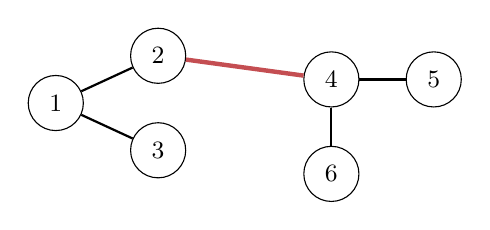
\begin{tikzpicture}
    \node[vtx] (1) at (0,0) {1};   \node[vtx] (2) at (1.3,0.6) {2};
    \node[vtx] (3) at (1.3,-0.6) {3};
    \node[vtx] (4) at (3.5,0.3) {4}; \node[vtx] (5) at (4.8,0.3) {5};
    \node[vtx] (6) at (3.5,-0.9) {6};
    \draw[thick] (1) -- (2); \draw[thick] (1) -- (3);
    \draw[thick] (4) -- (5); \draw[thick] (4) -- (6);
    \onslide<2->{\draw[line width=1.6pt, mRed] (2) -- (4);}
  \end{tikzpicture}
  \end{center}

  \begin{itemize}
    \item Is $3$ connected to $5$? \only<1>{No.}\only<2->{After adding the
          edge $\{2, 4\}$: \alert{yes}.}
    \item Rerunning DFS after each edge costs $O(n + m)$ per query. Too slow.
  \end{itemize}

  \medskip
  \onslide<3->{Used in Kruskal's minimum spanning tree algorithm, image
  segmentation, network connectivity, equivalence of variables in compilers,
  \ldots}
\end{frame}

\begin{frame}{The Disjoint-Set Interface}
  Maintain a partition of $\{1, \ldots, n\}$ into disjoint sets. Each set has
  one \alert{representative}.

  \medskip
  \begin{itemize}
    \item \texttt{find(x)}: return the representative of the set containing
          $x$.
    \item \texttt{union(x, y)}: merge the sets containing $x$ and $y$.
  \end{itemize}

  \medskip
  $x$ and $y$ are in the same set $\iff$ \texttt{find(x) == find(y)}.

  \bigskip
  \begin{center}
  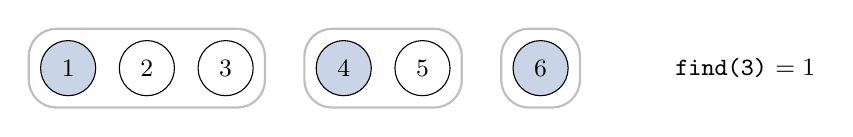
\begin{tikzpicture}
    \draw[blob] (-0.5,-0.5) rectangle (2.5,0.5);
    \draw[blob] (3,-0.5) rectangle (5,0.5);
    \draw[blob] (5.5,-0.5) rectangle (6.5,0.5);
    \node[root] at (0,0) {1}; \node[vtx] at (1,0) {2}; \node[vtx] at (2,0) {3};
    \node[root] at (3.5,0) {4}; \node[vtx] at (4.5,0) {5};
    \node[root] at (6,0) {6};
    \node[font=\small] at (8.6,0) {\texttt{find(3)} $= 1$};
  \end{tikzpicture}
  \end{center}

  \begin{center}
  \small Shaded vertices are the representatives.
  \end{center}
\end{frame}

\begin{frame}{First Attempt: Store the Label}
  Keep an array \texttt{label[x]} = representative of $x$.

  \bigskip
  \begin{center}
  \begin{tabular}{l|cccccc}
    $x$ & 1 & 2 & 3 & 4 & 5 & 6 \\ \hline
    \texttt{label[$x$]} & 1 & 1 & 1 & 4 & 4 & 6 \\
  \end{tabular}
  \end{center}

  \bigskip
  \begin{itemize}
    \item \texttt{find(x)}: return \texttt{label[x]}. \hfill $O(1)$
    \item \texttt{union(x, y)}: relabel every element whose label is
          \texttt{label[y]}. \hfill \alert{$O(n)$}
  \end{itemize}

  \pause
  \bigskip
  $n - 1$ unions cost $\Theta(n^2)$ in total. Can we make union cheap without
  making find expensive?
\end{frame}

% =========================================================================
\section{A Forest of Parent Pointers}

\begin{frame}{Sets as Trees}
  Store each set as a rooted tree. Every element points to its
  \alert{parent}. The root is the representative and points to itself.

  \bigskip
  \begin{columns}[c]
    \begin{column}{0.5\textwidth}
      \begin{center}
      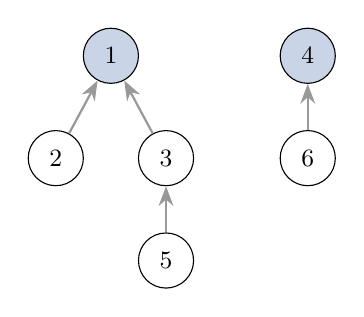
\begin{tikzpicture}
        \node[root] (1) at (1,1.5) {1};
        \node[vtx] (2) at (0.3,0.2) {2}; \node[vtx] (3) at (1.7,0.2) {3};
        \node[vtx] (5) at (1.7,-1.1) {5};
        \node[root] (4) at (3.5,1.5) {4}; \node[vtx] (6) at (3.5,0.2) {6};
        \draw[par] (2) -- (1); \draw[par] (3) -- (1); \draw[par] (5) -- (3);
        \draw[par] (6) -- (4);
      \end{tikzpicture}
      \end{center}
    \end{column}
    \begin{column}{0.45\textwidth}
      \begin{center}
      \parr{1}{1}{1}{4}{3}{4}
      \end{center}
    \end{column}
  \end{columns}

  \bigskip
  \begin{itemize}
    \item \texttt{find(x)}: follow parent pointers up to the root.
          Cost $=$ depth of $x$.
    \item \texttt{union(x, y)}: find both roots and make one point to the
          other. Cost $=$ two finds $+ O(1)$.
  \end{itemize}
\end{frame}

\begin{frame}[fragile]{Find and Union}
  \begin{columns}[c]
    \begin{column}{0.48\textwidth}
\begin{lstlisting}
function find(parent, x)
    while parent[x] != x
        x = parent[x]
    end
    return x
end

function union!(parent, x, y)
    rx = find(parent, x)
    ry = find(parent, y)
    if rx != ry
        parent[ry] = rx
    end
end
\end{lstlisting}
    \end{column}
    \begin{column}{0.48\textwidth}
      \begin{center}
      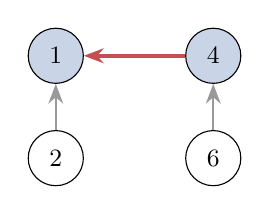
\begin{tikzpicture}
        \node[root] (1) at (0,1.3) {1};
        \node[vtx] (2) at (0,0) {2};
        \node[root] (4) at (2,1.3) {4};
        \node[vtx] (6) at (2,0) {6};
        \draw[par] (2) -- (1); \draw[par] (6) -- (4);
        \onslide<2->{\draw[new] (4) -- (1);}
      \end{tikzpicture}
      \end{center}
      \medskip
      \small \onslide<2->{\texttt{union!(parent, 2, 6)}: roots 1 and 4,
      so set \texttt{parent[4] = 1}.}
    \end{column}
  \end{columns}

  \medskip
  Initially \texttt{parent[x] = x} for every $x$: $n$ singleton trees.
\end{frame}

\begin{frame}{The Problem: Tall Trees}
  \texttt{union!(parent, 2, 1)}, \texttt{union!(parent, 3, 1)}, \ldots,
  \texttt{union!(parent, n, 1)}:

  \begin{columns}[c]
    \begin{column}{0.35\textwidth}
      \begin{center}
      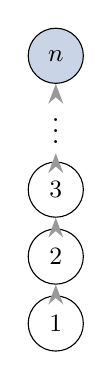
\begin{tikzpicture}[yscale=0.85]
        \node[root] (5) at (0,4) {$n$};
        \node (d) at (0,3) {$\vdots$};
        \node[vtx] (3) at (0,2) {3};
        \node[vtx] (2) at (0,1) {2};
        \node[vtx] (1) at (0,0) {1};
        \draw[par] (1) -- (2); \draw[par] (2) -- (3); \draw[par] (3) -- (d);
        \draw[par] (d) -- (5);
      \end{tikzpicture}
      \end{center}
    \end{column}
    \begin{column}{0.6\textwidth}
      \begin{itemize}
        \item Each union hangs the old tree below the new singleton.
        \item The tree becomes a path of height $n - 1$.
        \item \texttt{find(1)} now costs $\Theta(n)$, and $n$ such finds cost
              $\Theta(n^2)$.
      \end{itemize}

      \bigskip
      Two fixes:
      \begin{enumerate}
        \item \alert{Union by size}: keep trees shallow when merging.
        \item \alert{Path compression}: flatten trees when searching.
      \end{enumerate}
    \end{column}
  \end{columns}
\end{frame}

% =========================================================================
\section{Union by Size}

\begin{frame}[fragile]{Union by Size}
  Store \texttt{size[r]} = number of elements in the tree with root $r$.
  Always attach the \alert{smaller} tree below the root of the larger one.

  \begin{columns}[c]
    \begin{column}{0.5\textwidth}
\begin{lstlisting}
function union!(parent, size, x, y)
    rx = find(parent, x)
    ry = find(parent, y)
    rx == ry && return
    if size[rx] < size[ry]
        rx, ry = ry, rx   # rx is larger
    end
    parent[ry] = rx
    size[rx] += size[ry]
end
\end{lstlisting}
    \end{column}
    \begin{column}{0.45\textwidth}
      \begin{center}
      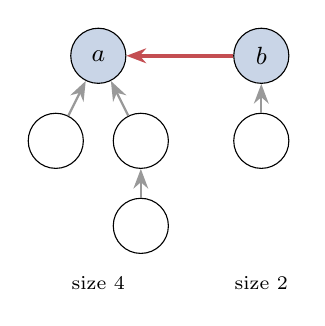
\begin{tikzpicture}[scale=0.9]
        \node[root] (a) at (0,1.2) {$a$};
        \node[vtx] (a1) at (-0.6,0) {}; \node[vtx] (a2) at (0.6,0) {};
        \node[vtx] (a3) at (0.6,-1.2) {};
        \draw[par] (a1) -- (a); \draw[par] (a2) -- (a); \draw[par] (a3) -- (a2);
        \node[font=\scriptsize] at (0,-2) {size 4};
        \node[root] (b) at (2.3,1.2) {$b$};
        \node[vtx] (b1) at (2.3,0) {};
        \draw[par] (b1) -- (b);
        \node[font=\scriptsize] at (2.3,-2) {size 2};
        \draw[new] (b) -- (a);
      \end{tikzpicture}
      \end{center}
      \small The size-2 tree goes below $a$. Ties: either way.
    \end{column}
  \end{columns}
\end{frame}

\begin{frame}{Union by Size Keeps Trees Shallow}
  \begin{block}{Lemma}
    With union by size, every tree of size $s$ has height at most
    $\log_2 s$. So every find costs $O(\log n)$.
  \end{block}

  \pause
  \textbf{Proof.} Follow one element $x$.
  \begin{itemize}
    \item The depth of $x$ grows by $1$ only when the root of its tree $T$ is
          attached below another root, whose tree $T'$ has
          $|T'| \ge |T|$.
    \item The merged tree has size $|T| + |T'| \ge 2|T|$: the size of the
          tree containing $x$ at least \alert{doubles}.
    \item The size starts at $1$ and never exceeds $s$, so this happens at
          most $\log_2 s$ times.
  \end{itemize}
  So every element has depth at most $\log_2 s$. \hfill $\square$

  \pause
  \medskip
  Union by \alert{rank} (an upper bound on height instead of size) gives the
  same guarantee.
\end{frame}

% =========================================================================
\section{Path Compression}

\begin{frame}{Path Compression}
  During \texttt{find(x)} we visit every vertex on the path from $x$ to the
  root. Make all of them point \alert{directly to the root}.

  \bigskip
  \begin{columns}[c]
    \begin{column}{0.45\textwidth}
      \begin{center}
      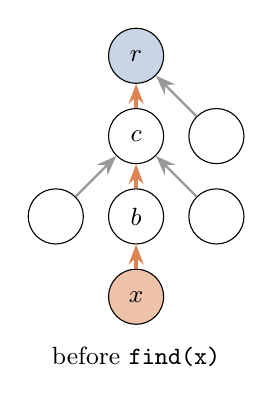
\begin{tikzpicture}[scale=0.85]
        \node[root] (r) at (0,3.6) {$r$};
        \node[vtx] (c) at (0,2.4) {$c$};
        \node[vtx] (b) at (0,1.2) {$b$};
        \node[hl] (x) at (0,0) {$x$};
        \node[vtx] (t1) at (1.2,2.4) {};
        \node[vtx] (t2) at (1.2,1.2) {};
        \node[vtx] (t3) at (-1.2,1.2) {};
        \draw[path] (x) -- (b); \draw[path] (b) -- (c); \draw[path] (c) -- (r);
        \draw[par] (t1) -- (r); \draw[par] (t2) -- (c); \draw[par] (t3) -- (c);
        \node[font=\small] at (0,-0.9) {before \texttt{find(x)}};
      \end{tikzpicture}
      \end{center}
    \end{column}
    \begin{column}{0.1\textwidth}
      \begin{center}\Large $\Rightarrow$\end{center}
    \end{column}
    \begin{column}{0.45\textwidth}
      \begin{center}
      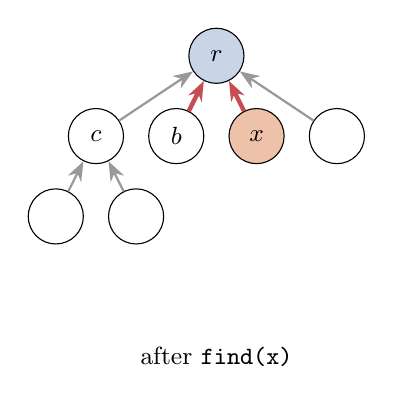
\begin{tikzpicture}[scale=0.85]
        \node[root] (r) at (0,3.6) {$r$};
        \node[vtx] (c) at (-1.8,2.4) {$c$};
        \node[vtx] (b) at (-0.6,2.4) {$b$};
        \node[hl] (x) at (0.6,2.4) {$x$};
        \node[vtx] (t1) at (1.8,2.4) {};
        \node[vtx] (t2) at (-2.4,1.2) {};
        \node[vtx] (t3) at (-1.2,1.2) {};
        \draw[new] (x) -- (r); \draw[new] (b) -- (r); \draw[par] (c) -- (r);
        \draw[par] (t1) -- (r); \draw[par] (t2) -- (c); \draw[par] (t3) -- (c);
        \node[font=\small] at (0,-0.9) {after \texttt{find(x)}};
      \end{tikzpicture}
      \end{center}
    \end{column}
  \end{columns}

  \bigskip
  The find costs the same this time, but every later find from $x$, $b$, or
  their descendants is faster.
\end{frame}

\begin{frame}[fragile]{Find with Path Compression}
  \begin{columns}[c]
    \begin{column}{0.48\textwidth}
\begin{lstlisting}
function find(parent, x)
    if parent[x] != x
        parent[x] = find(parent, parent[x])
    end
    return parent[x]
end
\end{lstlisting}
    \end{column}
    \begin{column}{0.48\textwidth}
      \begin{itemize}
        \item The recursion walks up to the root.
        \item On the way back, each vertex on the path gets the root as its
              new parent.
        \item One extra assignment per visited vertex, so the cost is still
              $O(\text{depth})$.
      \end{itemize}
    \end{column}
  \end{columns}

  \bigskip
  Path compression never changes the root of any set, so \texttt{size} only
  needs to be correct at the roots.
\end{frame}

\begin{frame}{Both Together}
  \begin{block}{Theorem (Tarjan, 1975)}
    With union by size (or rank) and path compression, any sequence of $m$
    operations on $n$ elements takes $O(m \, \alpha(n))$ time.
  \end{block}

  \bigskip
  \begin{itemize}
    \item $\alpha(n)$ is the \alert{inverse Ackermann function}. It grows
          absurdly slowly: $\alpha(n) \le 4$ for every $n$ smaller than the
          number of atoms in the universe.
    \item So in practice each operation is \alert{amortized constant} time.
    \item The proof is beyond this course; the $O(\log n)$ bound from union
          by size alone is the one to remember.
  \end{itemize}
\end{frame}

% =========================================================================
\section{Example}

% One overlay per step, fixed bounding box so slides do not jump
\begin{frame}{Example Trace}
  \small Union by size (ties: the root of $y$ goes below the root of $x$),
  path compression.

  \medskip
  \begin{center}
  \begin{tikzpicture}
    \useasboundingbox (-0.5,-2.6) rectangle (9.5,0.6);
    \only<1>{
      \foreach \i in {1,...,6} { \node[root] at (1.5*\i-1.5,0) {\i}; }
    }
    \only<2>{
      \node[root] (1) at (0,0) {1}; \node[vtx] (2) at (0,-1.2) {2};
      \draw[new] (2) -- (1);
      \foreach \i in {3,...,6} { \node[root] at (1.5*\i-3,0) {\i}; }
    }
    \only<3>{
      \node[root] (1) at (0,0) {1}; \node[vtx] (2) at (0,-1.2) {2};
      \node[root] (3) at (2,0) {3}; \node[vtx] (4) at (2,-1.2) {4};
      \draw[par] (2) -- (1); \draw[new] (4) -- (3);
      \node[root] at (4,0) {5}; \node[root] at (5.5,0) {6};
    }
    \only<4>{
      \node[root] (1) at (1,0) {1}; \node[vtx] (2) at (0,-1.2) {2};
      \node[vtx] (3) at (2,-1.2) {3}; \node[vtx] (4) at (2,-2.4) {4};
      \draw[par] (2) -- (1); \draw[new] (3) -- (1); \draw[par] (4) -- (3);
      \node[root] at (4,0) {5}; \node[root] at (5.5,0) {6};
    }
    \only<5>{
      \node[root] (1) at (1,0) {1}; \node[vtx] (2) at (0,-1.2) {2};
      \node[vtx] (3) at (2,-1.2) {3}; \node[vtx] (4) at (2,-2.4) {4};
      \draw[par] (2) -- (1); \draw[par] (3) -- (1); \draw[par] (4) -- (3);
      \node[root] (5) at (4.5,0) {5}; \node[vtx] (6) at (4.5,-1.2) {6};
      \draw[new] (6) -- (5);
    }
    \only<6>{
      \node[root] (1) at (2.25,0) {1};
      \node[vtx] (2) at (0,-1.2) {2}; \node[vtx] (3) at (1.5,-1.2) {3};
      \node[vtx] (4) at (3,-1.2) {4}; \node[vtx] (5) at (4.5,-1.2) {5};
      \node[vtx] (6) at (4.5,-2.4) {6};
      \draw[par] (2) -- (1); \draw[par] (3) -- (1);
      \draw[path] (4) -- (1); \draw[new] (5) -- (1); \draw[par] (6) -- (5);
    }
    \only<7>{
      \node[root] (1) at (3,0) {1};
      \node[vtx] (2) at (0,-1.2) {2}; \node[vtx] (3) at (1.5,-1.2) {3};
      \node[vtx] (4) at (3,-1.2) {4}; \node[vtx] (5) at (4.5,-1.2) {5};
      \node[vtx] (6) at (6,-1.2) {6};
      \draw[par] (2) -- (1); \draw[par] (3) -- (1); \draw[par] (4) -- (1);
      \draw[par] (5) -- (1); \draw[path] (6) -- (1);
    }
  \end{tikzpicture}
  \end{center}

  \medskip
  \begin{center}
  \only<1>{\parr{1}{2}{3}{4}{5}{6}}%
  \only<2>{\parr{1}{\nw{1}}{3}{4}{5}{6}}%
  \only<3>{\parr{1}{1}{3}{\nw{3}}{5}{6}}%
  \only<4>{\parr{1}{1}{\nw{1}}{3}{5}{6}}%
  \only<5>{\parr{1}{1}{1}{3}{5}{\nw{5}}}%
  \only<6>{\parr{1}{1}{1}{\nw{1}}{\nw{1}}{5}}%
  \only<7>{\parr{1}{1}{1}{1}{1}{\nw{1}}}%
  \end{center}

  \medskip
  \begin{center}
  \only<1>{Start: six singletons.}%
  \only<2>{\texttt{union(1, 2)}: sizes tie, so 2 goes below 1.}%
  \only<3>{\texttt{union(3, 4)}: 4 goes below 3.}%
  \only<4>{\texttt{union(2, 4)}: roots 1 and 3, both size 2, so 3 goes below 1.}%
  \only<5>{\texttt{union(5, 6)}: 6 goes below 5.}%
  \only<6>{\texttt{union(6, 4)}: \texttt{find(4)} compresses $4 \to 3 \to 1$
           (orange). Root 5 (size 2) goes below root 1 (size 4).}%
  \only<7>{\texttt{find(6)}: compresses $6 \to 5 \to 1$. Every element now
           points straight at the root.}%
  \end{center}
\end{frame}

\begin{frame}[fragile]{Union-Find in Julia}
  \begin{columns}[c]
    \begin{column}{0.55\textwidth}
\begin{lstlisting}[basicstyle=\ttfamily\scriptsize]
struct UnionFind
    parent::Vector{Int}
    size::Vector{Int}
end
UnionFind(n) = UnionFind(collect(1:n), ones(Int, n))
function find(uf::UnionFind, x)
    if uf.parent[x] != x
        uf.parent[x] = find(uf, uf.parent[x])
    end
    return uf.parent[x]
end
function union!(uf::UnionFind, x, y)
    rx, ry = find(uf, x), find(uf, y)
    rx == ry && return false
    if uf.size[rx] < uf.size[ry]; rx, ry = ry, rx; end
    uf.parent[ry] = rx
    uf.size[rx] += uf.size[ry]
    return true
end
\end{lstlisting}
    \end{column}
    \begin{column}{0.4\textwidth}
      \begin{itemize}
        \item The struct is immutable but its vectors are not, so
              \texttt{union!} can modify them.
        \item \texttt{union!} returns whether two different sets were
              merged. Kruskal's algorithm uses exactly this to decide
              whether to keep an edge.
      \end{itemize}
    \end{column}
  \end{columns}
\end{frame}

\begin{frame}[fragile]{Application: Counting Components}
  Count the connected components of an undirected graph with $n$ vertices and
  edge list \texttt{edges}.

  \begin{columns}[c]
    \begin{column}{0.5\textwidth}
\begin{lstlisting}
function count_components(n, edges)
    uf = UnionFind(n)
    count = n
    for (u, v) in edges
        if union!(uf, u, v)
            count -= 1
        end
    end
    return count
end
\end{lstlisting}
    \end{column}
    \begin{column}{0.45\textwidth}
      \begin{itemize}
        \item Start with $n$ components.
        \item Each edge joining two different sets merges two components.
        \item Time $O(n + m \, \alpha(n))$, and edges can be processed as
              they arrive.
      \end{itemize}
    \end{column}
  \end{columns}
\end{frame}

% =========================================================================
\begin{frame}{Exercise}
  Start with eight singletons $\{1\}, \ldots, \{8\}$. Use union by size
  (ties: the root of $y$ goes below the root of $x$) and path compression.

  \bigskip
  \begin{center}
  \texttt{union(1,2)}, \texttt{union(3,4)}, \texttt{union(5,6)},
  \texttt{union(7,8)}, \\
  \texttt{union(1,3)}, \texttt{union(5,7)}, \texttt{union(4,8)},
  \texttt{find(6)}
  \end{center}

  \bigskip
  \begin{enumerate}
    \item Draw the forest after the first six unions.
    \item Draw the forest after \texttt{union(4,8)}, and again after
          \texttt{find(6)}. Give the final \texttt{parent} array.
    \item Without path compression, what is the largest possible height of a
          tree on $8$ elements built by union by size?
  \end{enumerate}
\end{frame}

\begin{frame}{Solution}
  \begin{columns}[t]
    \begin{column}{0.33\textwidth}
      \centering\small (a) after six unions\\[4pt]
      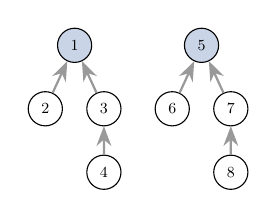
\begin{tikzpicture}[scale=0.62, every node/.append style={transform shape}]
        \node[root] (1) at (0.6,0) {1}; \node[vtx] (2) at (0,-1.3) {2};
        \node[vtx] (3) at (1.2,-1.3) {3}; \node[vtx] (4) at (1.2,-2.6) {4};
        \draw[par] (2) -- (1); \draw[par] (3) -- (1); \draw[par] (4) -- (3);
        \node[root] (5) at (3.2,0) {5}; \node[vtx] (6) at (2.6,-1.3) {6};
        \node[vtx] (7) at (3.8,-1.3) {7}; \node[vtx] (8) at (3.8,-2.6) {8};
        \draw[par] (6) -- (5); \draw[par] (7) -- (5); \draw[par] (8) -- (7);
      \end{tikzpicture}
    \end{column}
    \begin{column}{0.33\textwidth}
      \centering\small (b) after \texttt{union(4,8)}\\[4pt]
      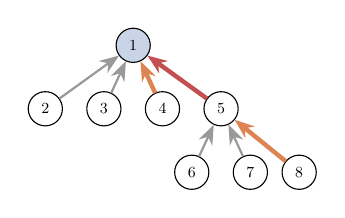
\begin{tikzpicture}[scale=0.62, every node/.append style={transform shape}]
        \node[root] (1) at (1.8,0) {1};
        \node[vtx] (2) at (0,-1.3) {2}; \node[vtx] (3) at (1.2,-1.3) {3};
        \node[vtx] (4) at (2.4,-1.3) {4}; \node[vtx] (5) at (3.6,-1.3) {5};
        \node[vtx] (6) at (3,-2.6) {6}; \node[vtx] (7) at (4.2,-2.6) {7};
        \node[vtx] (8) at (5.2,-2.6) {8};
        \draw[par] (2) -- (1); \draw[par] (3) -- (1); \draw[path] (4) -- (1);
        \draw[new] (5) -- (1);
        \draw[par] (6) -- (5); \draw[par] (7) -- (5); \draw[path] (8) -- (5);
      \end{tikzpicture}
    \end{column}
    \begin{column}{0.33\textwidth}
      \centering\small (b) after \texttt{find(6)}\\[4pt]
      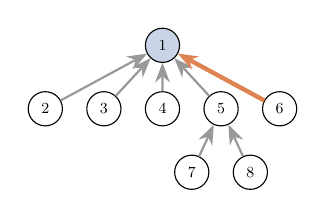
\begin{tikzpicture}[scale=0.62, every node/.append style={transform shape}]
        \node[root] (1) at (2.4,0) {1};
        \node[vtx] (2) at (0,-1.3) {2}; \node[vtx] (3) at (1.2,-1.3) {3};
        \node[vtx] (4) at (2.4,-1.3) {4}; \node[vtx] (5) at (3.6,-1.3) {5};
        \node[vtx] (6) at (4.8,-1.3) {6}; \node[vtx] (7) at (3,-2.6) {7};
        \node[vtx] (8) at (4.2,-2.6) {8};
        \draw[par] (2) -- (1); \draw[par] (3) -- (1); \draw[par] (4) -- (1);
        \draw[par] (5) -- (1); \draw[path] (6) -- (1);
        \draw[par] (7) -- (5); \draw[par] (8) -- (5);
      \end{tikzpicture}
    \end{column}
  \end{columns}

  \medskip
  \small
  In \texttt{union(4,8)}, \texttt{find(4)} compresses 4 onto 1 and
  \texttt{find(8)} compresses 8 onto 5; the sizes tie at 4, so 5 goes below 1.
  Final \texttt{parent} $= [1, 1, 1, 1, 1, 1, 5, 5]$.

  \medskip
  (c) $\log_2 8 = 3$, by the lemma. It is reached by merging equal-sized
  trees without compression: pairs, then pairs of pairs, then the two halves.
\end{frame}

% =========================================================================
\begin{frame}{Summary}
  \begin{center}
  \begin{tabular}{lcc}
    \toprule
    implementation & \texttt{find} & \texttt{union} \\
    \midrule
    label array & $O(1)$ & $O(n)$ \\
    parent forest, naive & $O(n)$ & $O(n)$ \\
    union by size & $O(\log n)$ & $O(\log n)$ \\
    union by size $+$ path compression & \multicolumn{2}{c}{$O(\alpha(n))$
      amortized} \\
    \bottomrule
  \end{tabular}
  \end{center}

  \bigskip
  \begin{itemize}
    \item Each set is a tree of parent pointers; its root is the
          representative.
    \item Union by size: attach the smaller tree, so heights stay
          $\le \log_2 n$.
    \item Path compression: point everything on a find path at the root.
  \end{itemize}
\end{frame}

\end{document}
